% Manual de usuario de PULSO: instalación, organización, aplicación, línea de comandos,
% configuración, datos, uso como biblioteca y solución de problemas.
% Compilar desde docs/latex/manual_usuario:
%   latexmk -lualatex manual_usuario.tex
\documentclass[11pt,a4paper,oneside]{report}

\usepackage{fontspec}
\usepackage[spanish,es-noshorthands,es-tabla,es-nodecimaldot]{babel}
\usepackage{amsmath,amssymb}
\setmainfont{TeX Gyre Pagella}
\setsansfont{TeX Gyre Heros}
\setmonofont{DejaVu Sans Mono}[Scale=0.82]
\usepackage[margin=2.3cm,headheight=14pt]{geometry}
\usepackage{graphicx}
\usepackage{booktabs,longtable,array}
\newcolumntype{L}[1]{>{\raggedright\arraybackslash}p{#1}}
\usepackage{xcolor}
\usepackage[most]{tcolorbox}
\usepackage{fvextra}
\usepackage{enumitem}
\usepackage{titlesec}
\usepackage{fancyhdr}
\usepackage{caption}
\usepackage{needspace}
\usepackage[hidelinks]{hyperref}

\graphicspath{{../figuras/manual/}{../figuras/}}

\definecolor{azul}{HTML}{2563A8}
\definecolor{rojo}{HTML}{C2362B}
\definecolor{verde}{HTML}{2F7D5B}
\definecolor{ambar}{HTML}{E0A100}
\definecolor{gris}{HTML}{5F6B77}

\titleformat{\chapter}[display]{\sffamily\bfseries\huge\color{azul}}
  {\large\chaptertitlename\ \thechapter}{6pt}{}
\titlespacing*{\chapter}{0pt}{-20pt}{20pt}
\titleformat{\section}{\sffamily\bfseries\Large}{\thesection}{0.7em}{}
\titleformat{\subsection}{\sffamily\bfseries\large}{\thesubsection}{0.7em}{}
\titleformat{\subsubsection}{\sffamily\bfseries\normalsize}{}{0em}{}

\pagestyle{fancy}
\fancyhf{}
\fancyhead[L]{\small\sffamily\color{gris}PULSO · manual de usuario}
\fancyhead[R]{\small\sffamily\color{gris}\nouppercase{\leftmark}}
\fancyfoot[C]{\small\thepage}
\renewcommand{\headrulewidth}{0.3pt}

\setlength{\parskip}{0.5em}
\setlength{\parindent}{0pt}
\setlength{\emergencystretch}{3em}
\setlist{itemsep=0.15em,topsep=0.25em}
\setlist[description]{font=\normalfont\bfseries,leftmargin=1.2em,labelindent=0em}
\captionsetup{font=small,labelfont=bf}

% Recuadros (los mismos del manual de la aplicación, que se incluye en el capítulo 5)
\newtcolorbox{pruebe}{colback=verde!6,colframe=verde,boxrule=0.5pt,arc=2pt,
  left=6pt,right=6pt,title={\sffamily\small Pruebe esto},coltitle=black,
  colbacktitle=verde!15,breakable,before upper={\setlength{\parskip}{0.4em}}}
\newtcolorbox{representa}{colback=azul!6,colframe=azul,boxrule=0.5pt,arc=2pt,
  left=6pt,right=6pt,title={\sffamily\small Qué representa},coltitle=black,
  colbacktitle=azul!15,breakable,before upper={\setlength{\parskip}{0.4em}}}
\newtcolorbox{aviso}{colback=ambar!8,colframe=ambar!80!black,boxrule=0.5pt,arc=2pt,
  left=6pt,right=6pt,title={\sffamily\small Tenga en cuenta},coltitle=black,
  colbacktitle=ambar!20,breakable,before upper={\setlength{\parskip}{0.4em}}}
\newenvironment{controles}{%
  \small\setlength{\LTpre}{0.3em}\setlength{\LTpost}{0.3em}
  \begin{longtable}{p{0.2\textwidth}p{0.17\textwidth}p{0.55\textwidth}}
  \toprule
  \textbf{Control} & \textbf{Rango (inicial)} & \textbf{Qué representa y qué pasa al
  cambiarlo} \\
  \midrule
  \endhead}{\bottomrule\end{longtable}}
\newcommand{\captura}[2][0.92]{%
  \begin{center}\fcolorbox{gris!40}{white}{\includegraphics[width=#1\textwidth]{#2}}\end{center}}
\newcommand{\boton}[1]{\fcolorbox{azul}{azul!10}{\sffamily\small #1}}

% Bloques de terminal y de archivos
\DefineVerbatimEnvironment{terminal}{Verbatim}{fontsize=\small,frame=single,
  framerule=0.4pt,rulecolor=\color{gris!50},framesep=3mm,breaklines=true,
  label=terminal,labelposition=topline}
\DefineVerbatimEnvironment{archivo}{Verbatim}{fontsize=\small,frame=single,
  framerule=0.4pt,rulecolor=\color{gris!50},framesep=3mm,breaklines=true,
  labelposition=topline}
\newcommand{\ruta}[1]{\texttt{\color{azul}#1}}

\hypersetup{pdftitle={PULSO: manual de usuario},pdfauthor={Juan Diego Martínez Ayala}}

\begin{document}

\begin{titlepage}
\centering
\vspace*{2.5cm}
{\sffamily\bfseries\Huge\color{azul} PULSO\par}
\vspace{0.2cm}
{\sffamily\large\color{gris} Pagos, Umbrales, Liquidez y Sincronización Operativa\par}
\vspace{0.9cm}
{\sffamily\LARGE Manual de usuario\par}
\vspace{0.4cm}
{\large Instalación, organización del proyecto, aplicación web, línea de comandos,\\
configuración, datos, uso como biblioteca y solución de problemas\par}
\vspace{1.2cm}
\fcolorbox{gris!40}{white}{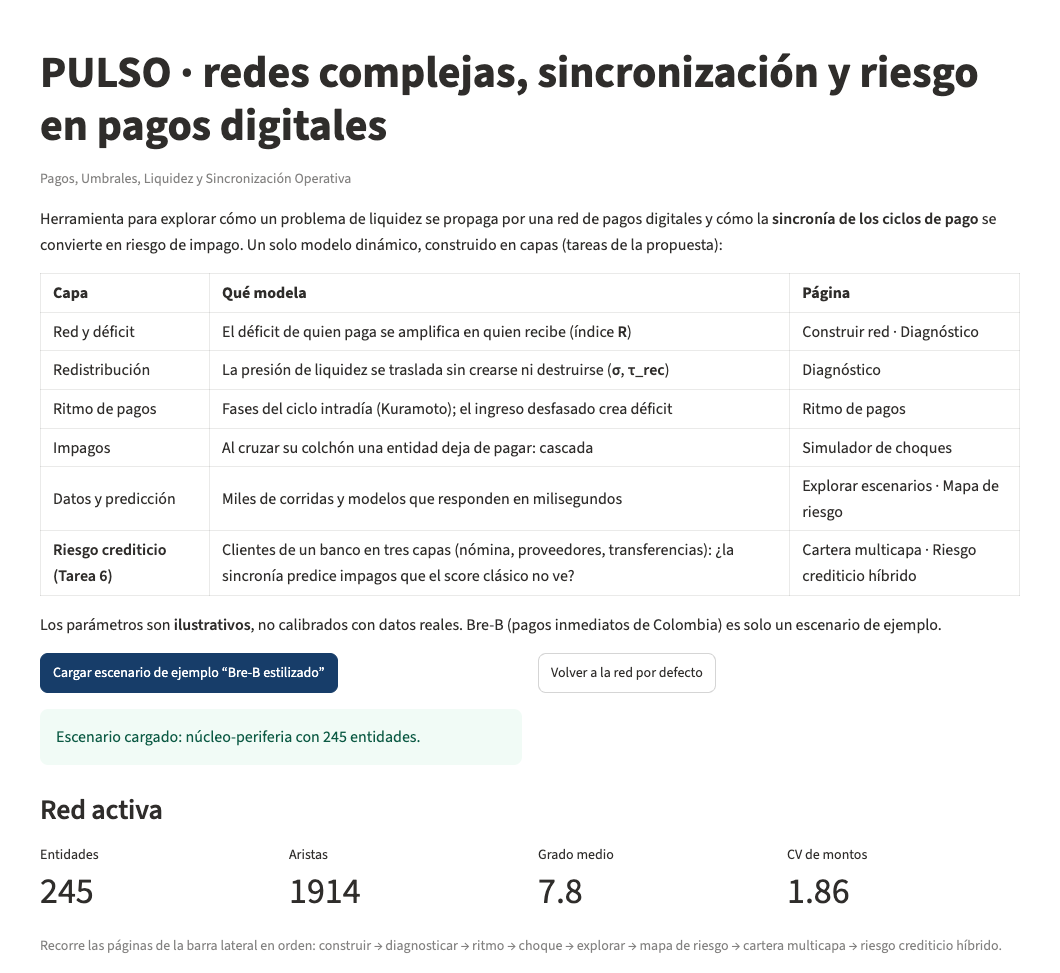
\includegraphics[width=0.66\textwidth]{inicio_1.png}}\par
\vfill
{\large Juan Diego Martínez Ayala\par}
{\normalsize Semillero de Modelamiento de Sistemas Complejos y Física Computacional\par}
\vspace{0.4cm}
{\normalsize Software versión 3.3.0 · noviembre de 2026\par}
\end{titlepage}

\tableofcontents

% ===================================================================
\chapter{Introducción}

\section{Qué es PULSO}
PULSO es un software para estudiar el riesgo en redes de pagos digitales. Modela cómo un
problema de liquidez se propaga entre entidades que se pagan entre sí, cómo se
sincronizan sus ciclos de pago y cuándo se producen cascadas de impagos. También aplica
ese modelo al riesgo de crédito de la cartera de un banco: estima, a partir de las
transacciones, si los ciclos de pago de cada cliente están sincronizados con los de
quienes le pagan, y usa esa información para predecir el impago.

El software tiene cuatro formas de uso:

\begin{center}
\begin{tabular}{p{0.26\textwidth}p{0.66\textwidth}}
\toprule
\textbf{Forma de uso} & \textbf{Para qué sirve} \\
\midrule
Aplicación web & Explorar el modelo de forma interactiva, sin programar
(capítulo~\ref{cap:app}). \\
Línea de comandos & Generar los datos, entrenar los modelos y correr el experimento de
crédito (capítulo~\ref{cap:cli}). \\
Biblioteca de Python & Usar las funciones del modelo en programas o notebooks propios
(sección~\ref{sec:biblioteca}). \\
Notebooks & Reproducir las figuras y el análisis de cada tarea
(\ruta{notebooks/}). \\
\bottomrule
\end{tabular}
\end{center}

\begin{aviso}
Todos los datos son sintéticos y los parámetros son ilustrativos, no calibrados con
información real. Los resultados sirven para estudiar mecanismos, no para medir el
riesgo de una institución concreta.
\end{aviso}

\section{A quién está dirigido este manual}
A quien instala, ejecuta o modifica el software. No supone conocimientos previos de
finanzas ni de redes: los conceptos necesarios se explican en la sección~\ref{sec:conceptos}.
Para el fundamento teórico completo, consulte la guía completa
(\ruta{docs/Presentaciones/v1/pulso\_guia\_completa.pdf}).

% ===================================================================
\chapter{Instalación}

\section{Requisitos}
\begin{center}
\begin{tabular}{p{0.24\textwidth}p{0.68\textwidth}}
\toprule
\textbf{Elemento} & \textbf{Requisito} \\
\midrule
Sistema operativo & macOS o Linux. En Windows, use Docker o WSL. \\
Python & 3.12 o superior (lo instala \texttt{uv} si no está). \\
uv & Gestor de entornos y dependencias: \url{https://docs.astral.sh/uv/}. \\
Espacio en disco & Unos 2 GB para el entorno (PyTorch ocupa la mayor parte). \\
Memoria & 8 GB recomendados. \\
Navegador & Cualquier navegador moderno, para la aplicación. \\
Docker (opcional) & Para ejecutar la aplicación sin instalar Python. \\
TeX Live (opcional) & Solo para regenerar los documentos PDF. \\
\bottomrule
\end{tabular}
\end{center}

\section{Instalación con uv}
En una terminal, dentro de la carpeta del proyecto:
\begin{terminal}
uv sync                       # crea el entorno .venv e instala las versiones exactas de uv.lock
uv run pytest -m "not slow"   # comprobación rápida: unas 107 pruebas en ~10 s
\end{terminal}
Si todas las pruebas pasan, la instalación es correcta. La batería completa, con las
pruebas lentas, se corre con \texttt{uv run pytest} y tarda alrededor de un minuto.

\section{Instalación con Docker}
\begin{terminal}
docker build -t pulso .
docker run -p 8501:8501 pulso
\end{terminal}
Abra \texttt{http://localhost:8501}. La imagen incluye los datos y los modelos ya
entrenados, así que la aplicación funciona sin correr ningún experimento.

\section{Primeros pasos}
\begin{enumerate}
\item Abra la aplicación:
\begin{terminal}
uv run streamlit run app/Inicio.py
\end{terminal}
Se abre \texttt{http://localhost:8501}. Para usar otro puerto, agregue
\texttt{--server.port=8502}.
\item En \emph{Inicio}, presione \boton{Cargar escenario de ejemplo “Bre-B estilizado”}.
\item Recorra las páginas en orden con la barra lateral.
\item Para cerrar la aplicación, presione \texttt{Ctrl+C} en la terminal.
\end{enumerate}

\begin{aviso}
En macOS, si el proyecto está dentro de \texttt{\textasciitilde/Documents}, puede aparecer
\texttt{ModuleNotFoundError: No module named 'pulso'}. La solución está en el
capítulo~\ref{cap:problemas}.
\end{aviso}


% ===================================================================
\chapter{Organización del proyecto}

\section{Mapa de carpetas}
\begin{archivo}[label=estructura]
pulso/
├── README.md               qué es el proyecto, resultados y cómo usarlo
├── CHANGELOG.md            historial de versiones
├── pyproject.toml          ficha del paquete: nombre, versión, dependencias, comando pulso
├── uv.lock                 versiones exactas de todas las dependencias
├── .python-version         versión de Python (3.12)
├── Dockerfile              receta de la imagen de la aplicación
├── .dockerignore           lo que no entra en la imagen
├── .gitignore              lo que git no guarda (entorno, cachés, temporales)
├── .github/workflows/ci.yml   integración continua: ruff, pytest y Docker
├── .streamlit/config.toml  tema y opciones del servidor de la aplicación
├── configs/                TODOS los parámetros, en YAML
├── src/pulso/              el código del modelo (paquete de Python)
├── app/                    la aplicación web (Streamlit)
├── data/                   datos generados por los experimentos
├── models/                 modelos entrenados y versionados
├── figures/                figuras de las tareas 1 a 6
├── notebooks/              análisis y figuras de cada tarea
├── tests/                  pruebas automáticas
└── docs/                   documentación, fuentes LaTeX y PDF
\end{archivo}

La regla del proyecto es separar responsabilidades: los \textbf{parámetros} viven en
\ruta{configs/}, el \textbf{cálculo} en \ruta{src/pulso/}, la \textbf{presentación} en
\ruta{app/} y los \textbf{resultados} en \ruta{data/}, \ruta{models/} y
\ruta{figures/}. Ningún número del modelo está escrito en el código.

\section{El código: \texttt{src/pulso/}}

\subsection*{Núcleo del modelo (tareas 1 a 4)}
\begin{longtable}{L{0.24\textwidth}L{0.68\textwidth}}
\toprule
\textbf{Archivo} & \textbf{Qué hace} \\
\midrule
\endhead
\texttt{networks.py} & Genera redes de pagos: Erdős–Rényi, Barabási–Albert y
núcleo-periferia, con montos lognormales escalados a media 1. \\
\texttt{model.py} & Define los parámetros del modelo (\texttt{Params}), los colchones
de impago y el lado derecho de las ecuaciones de déficit y fase, incluido el
acoplamiento multicapa. \\
\texttt{integrate.py} & Integra las ecuaciones en el tiempo (Runge–Kutta 4, ruido de
Euler–Maruyama), aplica choques y detecta impagos y cascadas. \\
\texttt{spectral.py} & Análisis espectral: radio espectral, índice $R$, estabilidad
$\sigma$, tiempo de recuperación, $\lambda_2$, comunidades y ranking de entidades. \\
\texttt{cascades.py} & Modelos clásicos de contagio para comparar: Eisenberg–Noe,
DebtRank y Watts. \\
\texttt{metrics.py} & Indicadores de cada simulación: fracción en impago, liquidez no
pagada, primer contagio, colapso e importancia sistémica. \\
\bottomrule
\end{longtable}

\subsection*{Experimentos y predicción (tarea 5)}
\begin{longtable}{L{0.24\textwidth}L{0.68\textwidth}}
\toprule
\textbf{Archivo} & \textbf{Qué hace} \\
\midrule
\endhead
\texttt{experiments.py} & Barrido de escenarios: muestrea redes y parámetros, simula y
guarda las tablas con su esquema validado. \\
\texttt{ml/train.py} & Entrena y valida (GroupKFold por red) la regresión logística,
XGBoost y la GCN; guarda métricas. \\
\texttt{ml/gnn.py} & Red neuronal sobre grafos (GCN) con conexión residual. \\
\texttt{ml/pinn.py} & Red neuronal informada por la física para estimar parámetros. \\
\texttt{ml/predict.py} & Predicción instantánea para una red nueva, explicación SHAP y
verificación por simulación. \\
\texttt{ml/registry.py} & Guarda y carga modelos con versión y metadatos. \\
\bottomrule
\end{longtable}

\subsection*{Cartera de un banco (tarea 6)}
\begin{longtable}{L{0.24\textwidth}L{0.68\textwidth}}
\toprule
\textbf{Archivo} & \textbf{Qué hace} \\
\midrule
\endhead
\texttt{world/schema.py} & Constantes (tipos de cliente, capas) y esquemas de las tablas
de la cartera. \\
\texttt{world/entities.py} & Genera personas y empresas con sus variables y su
probabilidad de impago verdadera. \\
\texttt{world/layers.py} & Genera las relaciones de nómina, proveedores y
transferencias. \\
\texttt{world/core.py} & Reúne todo en un objeto \texttt{World}; lo guarda y lo carga. \\
\texttt{world/transactions.py} & Convierte la simulación en un registro de
transacciones como el de un banco. \\
\texttt{credit/engine.py} & Parámetros y simulación del modelo multicapa, colchones según
la PD e impagos idiosincráticos. \\
\texttt{credit/estimate.py} & Estima la red, las fases y la coherencia a partir de las
transacciones. \\
\texttt{credit/features.py} & Calcula las variables de cada cliente en tres niveles:
clásico, red estática y red dinámica. \\
\texttt{credit/pipeline.py} & Une generación, simulación, transacciones y variables para
una cartera. \\
\texttt{credit/evaluate.py} & Validación cruzada por cartera, métricas, diferencias
pareadas e intervalos de confianza. \\
\texttt{credit/experiment.py} & Experimento completo de la tarea 6: carteras, regímenes,
resultados y modelos finales. \\
\texttt{credit/service.py} & Funciones que usa la aplicación en las páginas 8 y 9. \\
\bottomrule
\end{longtable}

\subsection*{Utilidades}
\begin{longtable}{L{0.24\textwidth}L{0.68\textwidth}}
\toprule
\textbf{Archivo} & \textbf{Qué hace} \\
\midrule
\endhead
\texttt{config.py} & Lee los YAML de \ruta{configs/} y resuelve las carpetas de datos y
modelos (admite variables de entorno). \\
\texttt{schema.py} & Valida columnas, tipos y rangos de las tablas, y prohíbe usar las
columnas de verdad \texttt{truth\_*}. \\
\texttt{service.py} & Funciones que usa la aplicación en las páginas 1 a 7. \\
\texttt{viz.py} & Gráficas interactivas (Plotly) de la aplicación. \\
\texttt{cli.py} & El comando \texttt{pulso} (capítulo~\ref{cap:cli}). \\
\bottomrule
\end{longtable}

\section{Las demás carpetas}
\begin{longtable}{L{0.3\textwidth}L{0.62\textwidth}}
\toprule
\textbf{Carpeta o archivo} & \textbf{Contenido} \\
\midrule
\endhead
\ruta{app/Inicio.py} & Página de inicio de la aplicación. \\
\ruta{app/common.py} & Estado compartido y cachés de la aplicación. \\
\ruta{app/pages/1\_…9\_*.py} & Una página por archivo (capítulo~\ref{cap:app}). \\
\ruta{configs/*.yaml} & Parámetros (capítulo~\ref{cap:config}). \\
\ruta{data/*.parquet}, \texttt{networks.npz} & Conjunto de datos de la tarea 5; ficha en
\ruta{data/README.md}. \\
\ruta{data/credit/} & Resultados del experimento de la tarea 6. \\
\ruta{models/} & Modelos de la tarea 5 por nombre y versión; \ruta{models/credit/v1/}
para la tarea 6. \\
\ruta{figures/} & Figuras de los notebooks y de la aplicación. \\
\ruta{notebooks/01…06} & Un notebook por tarea, del 01 (red y déficit) al 06 (PINN). \\
\ruta{tests/test\_fase*.py} & Pruebas por fase; \texttt{test\_app.py} prueba que cada
página de la aplicación se ejecute sin errores. \\
\ruta{docs/Presentaciones/} & PDF finales: v1, v2, v3, manuales y plan de estudio. \\
\ruta{docs/latex/} & Fuentes LaTeX, generador de figuras (\texttt{figuras.py}) y
\texttt{compilar.sh}. \\
\ruta{docs/diseno/} & Especificación de diseño de la tarea 6. \\
\ruta{docs/bibliografia.md} & Referencias por tarea. \\
\bottomrule
\end{longtable}

\begin{aviso}
No se guardan en git: el entorno (\ruta{.venv/}), las cachés de Python y la tabla
grande de clientes \ruta{data/credit/clientes.parquet}, que se regenera con
\texttt{uv run pulso credit configs/credit.yaml}.
\end{aviso}


\chapter{La aplicación web}
\label{cap:app}
Este capítulo describe cada página de la aplicación: qué representa, qué hace cada
control y cómo leer cada resultado. Empieza con los elementos comunes a todas las páginas.

\section{Elementos de la pantalla}
\label{sec:pantalla}
\begin{description}
\item[Barra lateral.] A la izquierda. Tiene la lista de páginas y, debajo, un resumen de
la red activa o de la cartera activa. Se oculta con la flecha \texttt{<<}.
\item[Deslizador.] Barra con un punto que se arrastra para elegir un número. El valor
actual aparece encima.
\item[Formulario.] Recuadro con varios controles y un botón azul (\boton{Construir},
\boton{Simular}, \boton{Simular cartera}). Los cambios no se aplican hasta presionar el
botón.
\item[Métrica.] Número grande con su nombre encima. El símbolo \textbf{?} muestra una
explicación al pasar el cursor. Debajo puede aparecer la diferencia frente a un caso de
referencia.
\item[Gráfica interactiva.] Muestra información al pasar el cursor. Se amplía
arrastrando un rectángulo; doble clic restablece la vista. Los botones de la esquina
permiten descargar la imagen. Un clic en la leyenda oculta o muestra una serie.
\item[Tabla.] Un clic en el nombre de una columna la ordena.
\item[Desplegable.] Línea con una flecha \texttt{>} que muestra contenido adicional.
\item[Indicador de ejecución.] Aparece arriba a la derecha mientras la aplicación calcula.
\end{description}

\subsection{Estado compartido y límites}
\begin{itemize}
\item La red construida en \emph{Construir red} y los parámetros elegidos en
\emph{Diagnóstico}, \emph{Ritmo de pagos} y \emph{Simulador de choques} se comparten entre
las páginas 1 a 7. La cartera de \emph{Cartera multicapa} se comparte con la página 9.
\item El estado dura mientras la pestaña del navegador esté abierta. Al recargarla, todo
vuelve a los valores iniciales.
\item Con más de 300 entidades se desactivan las simulaciones en vivo; el \emph{Mapa de
riesgo} sigue funcionando porque predice sin simular. El límite está en
\texttt{configs/default.yaml} (\texttt{app.max\_live\_entities}).
\end{itemize}

\subsection{Conceptos mínimos}
\label{sec:conceptos}
\begin{description}
\item[Entidad o nodo.] Participante de la red: un banco, una empresa o una persona.
\item[Arista.] Pago recurrente de una entidad a otra. Su peso es el pago medio por ciclo.
\item[Ciclo.] Unidad de tiempo de las páginas 1 a 7 (un día hábil). En las páginas 8 y 9
la unidad es el mes.
\item[Déficit.] Liquidez que le falta a una entidad.
\item[Colchón.] Déficit máximo que soporta antes de dejar de pagar.
\item[Impago y cascada.] Una entidad deja de pagar; si eso lleva a otras a dejar de pagar,
se produce una cascada.
\item[Fase y sincronía.] Momento del ciclo de pagos en que está una entidad, y qué tan
alineados están los ciclos de todas.
\item[PD.] Probabilidad de impago de un cliente en los próximos doce meses.
\item[Semilla.] Número que fija el azar: con la misma semilla se obtiene el mismo
resultado.
\end{description}

% ===================================================================
\section{Inicio}

\captura{inicio_1.png}

La página de inicio resume el modelo en una tabla. Cada fila es una capa del modelo,
lo que modela y la página donde se explora.

\begin{description}
\item[\boton{Cargar escenario de ejemplo “Bre-B estilizado”}.] Reemplaza la red y los
parámetros por un escenario de ejemplo: red núcleo-periferia de 245 entidades (del orden
de los participantes de Bre-B en su primer año), grado medio 8, índice de amplificación
$R=0.85$, redistribución $D_0=0.05$, acople $K=3$ y colchón $0.5$. Los valores son
ilustrativos.
\item[\boton{Volver a la red por defecto}.] Restaura la red inicial: núcleo-periferia de
80 entidades, grado medio 6, $R=0.8$, semilla 42.
\end{description}

Debajo, cuatro métricas describen la red activa:

\begin{description}
\item[Entidades.] Número de nodos.
\item[Aristas.] Número de relaciones de pago dirigidas.
\item[Grado medio.] Número medio de pagadores (o de receptores) por entidad.
\item[CV de montos.] Coeficiente de variación de los montos: desviación estándar
dividida por la media. Un valor alto indica pocos pagos muy grandes y muchos pequeños.
\end{description}

% ===================================================================
\section{Construir red}

\captura{construir_1.png}

\begin{representa}
Un sistema de pagos como red. Cada círculo es una entidad y cada línea un pago
recurrente. El tamaño del círculo es proporcional al volumen de pagos. En la topología
núcleo-periferia, los círculos rojos son el núcleo: las grandes entidades que concentran
los pagos.
\end{representa}

\subsection*{Controles (dentro del formulario)}
\begin{controles}
Topología & Erdős–Rényi, Barabási–Albert, Núcleo-periferia (núcleo-periferia) &
Forma de la red. \textbf{Erdős–Rényi}: conexiones al azar, todas las entidades parecidas.
\textbf{Barabási–Albert}: unas pocas entidades muy conectadas (concentradores).
\textbf{Núcleo-periferia}: un núcleo denso y una periferia conectada a él; es la forma de
los sistemas de pagos reales. \\
Número de entidades & 10 a 600 (80) & Tamaño de la red. Por encima de 300 se desactiva la
simulación en vivo. \\
Grado medio & 1 a 20 (6) & Número medio de contrapartes de cada entidad. Más grado, red
más densa. Debe ser menor que el número de entidades menos uno. \\
Dispersión de montos ($\sigma$ lognormal) & 0 a 2 (0.8) & Desigualdad de los montos. Con
0 todos los pagos valen igual; con valores altos aparecen pagos muy grandes. \\
Fracción en el núcleo & 0.02 a 0.40 (0.10) & Proporción de entidades del núcleo. Solo se
activa con núcleo-periferia. \\
Semilla & 0 a $10^6$ (42) & Fija el azar de la construcción. Cambiarla produce otra red
con las mismas características. \\
\end{controles}

Al presionar \boton{Construir} se genera la red. Las simulaciones previas se borran
porque correspondían a la red anterior.

\subsection*{Resultados}
\begin{description}
\item[Entidades y aristas dirigidas.] Tamaño de la red.
\item[Densidad.] Fracción de las conexiones posibles que existen, entre 0 y 1.
\item[CV de montos.] Ver \emph{Inicio}.
\item[Gráfica de la red.] Al pasar el cursor sobre una entidad se ve cuánto paga y
cuánto recibe por ciclo.
\end{description}

\begin{pruebe}
Construya una red Barabási–Albert de 100 entidades y luego una Erdős–Rényi del mismo
tamaño y grado. En la primera verá unos pocos círculos grandes en el centro; en la
segunda, círculos de tamaño parecido. Después vaya a \emph{Diagnóstico}: con el mismo
$\beta$, la red Barabási–Albert tendrá un $R$ mayor.
\end{pruebe}

% ===================================================================
\section{Diagnóstico}

\captura{diagnostico_1.png}

\begin{representa}
La salud de la red frente a un choque, calculada sin simular, a partir de los valores
propios de la red. Responde: si una entidad sufre un déficit, ¿la red lo absorbe o lo
amplifica? ¿Cuánto tarda en recuperarse? ¿Qué entidades son más importantes?
\end{representa}

\subsection*{Controles}
\begin{controles}
$\alpha$ · autocorrección [1/ciclo] & 0.05 a 3 (1.0) & Rapidez con que cada entidad
corrige su déficit por sí misma. $1/\alpha$ es el tiempo típico de corrección. Subirlo
estabiliza la red. \\
$\beta$ · amplificación & 0 a $2\alpha/\rho$ (el que da $R=0.8$) & Déficit que genera en
una entidad el déficit de quien le paga. El rango se ajusta a la red para que $R$ vaya de
0 a 2. Subirlo desestabiliza la red. \\
$D_0$ · redistribución & 0 a 2 (0) & Traslado de presión de liquidez de una entidad a sus
receptores sin crearla ni destruirla. Acelera la recuperación. \\
Comunidades & 2 a 8 (3) & Número de grupos en que se divide la red para colorearla. \\
\end{controles}

\subsection*{Resultados}
\begin{description}
\item[Índice de amplificación $R$.] $R=\beta\rho(W)/\alpha$, donde $\rho(W)$ es el radio
espectral de la red (su valor propio dominante). $R<1$: la red amortigua. $R>1$: la red
amplifica. Es el análogo del número reproductivo de una epidemia.
\item[Estabilidad $\sigma$ con semáforo.] Mayor parte real de los valores propios de
$M=-\alpha I-D_0L+\beta W$. Incluye la redistribución, así que es más completo que $R$.
\textcolor{verde}{Verde}: $\sigma<-0.05$, la red amortigua.
\textcolor{ambar}{Amarillo}: $|\sigma|\le0.05$, la red está cerca del límite y los
choques tardan mucho en disiparse. \textcolor{rojo}{Rojo}: $\sigma>0.05$, el déficit
crece sin límite.
\item[Tiempo de recuperación.] $\tau_\text{rec}=-1/\sigma$, en ciclos: tiempo en que un
choque se reduce a un 37~\% ($1/e$). Aparece $\infty$ si la red no se recupera.
\item[Conectividad algebraica $\lambda_2$.] Mide qué tan bien conectada está la red como
un todo. Vale 0 si está partida en pedazos aislados. Mayor $\lambda_2$, más rápida la
redistribución.
\item[Comunidades.] Gráfica con la red coloreada por grupos que se pagan mucho entre sí y
poco con el resto. Se obtienen con el vector de Fiedler (bisección espectral).
\item[Ranking por vector propio dominante.] Las 15 entidades más importantes.
\emph{importancia}: cuánto déficit propaga si entra en problemas (vector propio
izquierdo). \emph{vulnerabilidad}: cuánto déficit acumula si otros entran en problemas
(vector propio derecho). \emph{paga} y \emph{recibe}: flujos por ciclo.
\end{description}

\captura{diagnostico_2.png}

\subsection*{Choque de prueba (sin impagos)}
Aplica un retiro de liquidez a una entidad y muestra cómo evoluciona el déficit, sin
umbrales: nadie entra en impago. Sirve para ver la estabilidad en acción.

\begin{controles}
Entidad chocada & 0 a $n-1$ (la más importante) & Entidad que sufre el choque. \\
Tamaño & 0.1 a 10 ciclos (2) & Déficit inicial, medido en ciclos de los pagos salientes
de la entidad: 2 equivale a dos ciclos de lo que paga. \\
\end{controles}

\begin{description}
\item[Trayectorias.] El déficit de cada entidad en el tiempo; la entidad chocada aparece
resaltada.
\item[Déficit total del sistema ($\Sigma x$).] Suma de todos los déficits. Con $R<1$
termina en cero; con $R>1$ crece.
\end{description}

\begin{pruebe}
Mueva $\beta$ hasta que $R$ pase de 0.9 a 1.1. El semáforo cambia de verde a rojo y el
déficit total del choque de prueba deja de bajar y empieza a crecer. Luego suba $D_0$:
$\sigma$ baja y la red puede volver a ser estable aunque $R>1$.
\end{pruebe}

% ===================================================================
\section{Ritmo de pagos}

\captura{ritmo_1.png}

\begin{representa}
Cada entidad paga en ciclos, como un reloj que da vueltas. La posición en la vuelta es
su fase. Cada entidad tiene su propio ritmo, pero tiende a ajustarlo al de quienes le
pagan. La página muestra si las entidades terminan sincronizadas y cuánto déficit se
genera cuando el ingreso llega desfasado.
\end{representa}

\subsection*{Controles}
\begin{controles}
$K$ · dependencia de fondos entrantes & 0 a 10 (2) & Intensidad con que cada entidad
ajusta su ritmo al de quienes le pagan. Más $K$, más sincronía. \\
$\Delta$ · dispersión de ritmos naturales & 0 a 2 (0.5) & Qué tan distintos son los
ritmos propios de las entidades. Más $\Delta$, más difícil sincronizar. \\
$\gamma$ · peso de la desincronización en el déficit & 0 a 0.5 (0) & Cuánto déficit genera
el ingreso desfasado. Con 0, la sincronía no afecta la liquidez. \\
Desconectar entidad a mitad de la corrida & ninguna o una de las 30 que más pagan &
Elimina todos los pagos de esa entidad en la mitad de la simulación (ciclo 10 de 20). \\
\end{controles}

\subsection*{Resultados}
\begin{description}
\item[$r$ final.] Parámetro de orden al final: 0 si las fases están dispersas, 1 si todas
coinciden. Con una desconexión, la flecha muestra la diferencia frente a la red
completa.
\item[Déficit total final.] Suma de los déficits al final. Con desconexión, muestra la
diferencia.
\item[Coherencia local media.] Promedio de $r_i$, que mide si a cada entidad le llega el
ingreso en fase (1), sin relación (0) o en contrafase ($-1$).
\item[Círculo de fases.] Animación: cada punto es una entidad sobre un círculo según su
fase. Si se agrupan, están sincronizadas. Use el botón de reproducción.
\item[Parámetro de orden $r(t)$.] Evolución de la sincronía. Con desconexión se muestran
dos curvas: con y sin la entidad.
\item[Déficit total.] Evolución de la suma de déficits.
\item[Coherencia local al final.] Red coloreada por $r_i$: verde, ingreso en fase; rojo,
en contrafase.
\end{description}

\captura[0.8]{ritmo_2.png}

\begin{aviso}
Con $\gamma=0$ aparece un mensaje: las fases se sincronizan, pero el déficit no cambia.
Suba $\gamma$ para ver el efecto del ritmo sobre la liquidez.
\end{aviso}

\begin{pruebe}
Con $\gamma=0.1$, mueva $K$ de 0 a 6. Con $K$ bajo, $r$ queda cerca de 0 y el déficit
total crece; con $K$ alto, $r$ se acerca a 1 y el déficit se reduce. Después desconecte la
primera entidad de la lista: $r$ cae y el déficit sube en la segunda mitad.
\end{pruebe}

% ===================================================================
\section{Simulador de choques}

\captura{simulador_1.png}

\begin{representa}
Un choque sobre una entidad y la cascada de impagos que provoca. A diferencia del
choque de prueba de \emph{Diagnóstico}, aquí sí hay colchones: la entidad que los supera
deja de pagar y sus receptores pierden ingreso. Usa los parámetros $\alpha$, $\beta$,
$D_0$, $K$ y $\gamma$ elegidos en las páginas anteriores.
\end{representa}

\subsection*{Controles (dentro del formulario)}
\begin{controles}
Entidad chocada & todas, ordenadas por lo que pagan & Entidad que recibe el choque. Junto
al número aparece cuánto paga por ciclo. \\
Tipo de choque & Retiro de liquidez o Caída operativa & \textbf{Retiro de liquidez}: un
salto súbito en el déficit, como una retirada masiva de depósitos. \textbf{Caída
operativa}: la entidad sigue recibiendo pero no paga durante un tiempo, como una falla
tecnológica. \\
Tamaño del retiro & 0.1 a 10 ciclos (2) & Solo para el retiro: déficit inicial en ciclos
de pagos salientes. \\
Duración de la caída $T$ & 0.5 a 15 ciclos (3) & Solo para la caída operativa: cuánto
dura sin pagar. \\
Colchón $c$ & 0.05 a 3 (0.5) & Reserva de cada entidad, medida en ciclos de sus pagos
salientes. Más colchón, menos impagos. \\
$\lambda$ · pérdida por ingreso no recibido & 0 a 3 (1) & Cuánto déficit genera perder un
pagador. Con 1, perder todo el ingreso equivale a un ciclo de los pagos propios. \\
\end{controles}

El choque ocurre en el ciclo 1 y la simulación dura 20 ciclos.

\subsection*{Resultados}
\begin{description}
\item[En impago.] Porcentaje de entidades que terminan en impago. El símbolo \textbf{?}
muestra el número.
\item[Liquidez no pagada.] Pagos que no se hicieron por los impagos, acumulados, en pagos
medios.
\item[DebtRank.] Medida clásica del daño sistémico (Battiston et al., 2012), entre 0 y
1: fracción del valor económico de la red afectada por el estrés, sin contar a la
entidad chocada.
\item[Primer contagio.] Ciclo en que cae la primera entidad distinta de la chocada.
``—'' si no hubo contagio.
\item[Colapso global.] Mensaje rojo si cae el 30~\% o más de la red.
\item[Animación de la cascada.] Red coloreada por estado: \textcolor{verde}{verde}, sin
problemas; \textcolor{ambar}{ámbar}, en estrés (déficit mayor que la mitad de su
colchón); \textcolor{rojo}{rojo}, en impago. La entidad chocada tiene borde negro. Use el
botón de reproducción o arrastre la barra de tiempo.
\item[Línea de tiempo de eventos.] Cada punto es un impago: en el eje horizontal el
ciclo y en el vertical la entidad.
\item[Liquidez no pagada acumulada.] Evolución en el tiempo del indicador anterior.
\item[\boton{Exportar indicadores y eventos (CSV)}.] Descarga los resultados en un
archivo que se abre con Excel.
\end{description}

\begin{aviso}
Si $\gamma>0$ algunas entidades pueden caer antes del choque por la desincronización.
Un mensaje lo indica; esas caídas no cuentan como contagio.
\end{aviso}

\captura{simulador_2.png}

\subsection*{Entidades más peligrosas}
El botón \boton{Calcular ranking} choca, una por una, cada entidad con el tamaño elegido
y mide la fracción media de las demás que caen (\emph{cascada\_media}). Muestra las 10 más
peligrosas. Tarda unos segundos y el resultado queda guardado mientras no cambie la
configuración.

\begin{pruebe}
Choque la entidad que más paga con un retiro de 3 ciclos y colchón 0.5. Anote el
porcentaje en impago. Suba el colchón a 1.0 y repita: la cascada se reduce mucho.
Luego compare un retiro con una caída operativa de 3 ciclos sobre la misma entidad.
\end{pruebe}

% ===================================================================
\section{Explorar escenarios}

\captura{explorar_1.png}

\begin{representa}
Los resultados de 20\,000 simulaciones hechas de antemano sobre 300 redes distintas,
con parámetros variados. Permite responder preguntas generales sin simular: ¿en qué
condiciones colapsa una red? ¿Qué topología es más frágil?
\end{representa}

\begin{aviso}
Requiere el conjunto de datos. Si no existe, la página indica el comando para generarlo:
\texttt{uv run pulso sweep configs/sweep.yaml} (unos 20 minutos).
\end{aviso}

\subsection*{Filtros (en el desplegable \emph{Filtros})}
\begin{controles}
Topología & las tres (todas) & Redes que se incluyen. \\
Tipo de choque & liquidez, operativo (ambos) & Choques que se incluyen. \\
Índice de amplificación $R$ & 0.4 a 1.6 (todo) & Rango de $R$. \\
Grado medio & 2 a 12 (todo) & Rango de conectividad. \\
Colchón $c$ & 0.2 a 1.5 (todo) & Rango de colchones. \\
Acople $K$ & 0 a 6 (todo) & Rango de acople de fase. \\
\end{controles}

\subsection*{Resultados}
\begin{description}
\item[Corridas filtradas.] Número de simulaciones que cumplen los filtros.
\item[P(colapso).] Porcentaje de ellas con colapso global (30~\% o más en impago).
\item[Fracción media en impago.] Promedio del porcentaje de entidades que caen.
\item[Liquidez no pagada media.] En ciclos de flujo total del sistema.
\item[Ventana de contagio.] Fracción en impago contra grado medio, por topología. Muestra
que las cascadas son mayores con conectividad intermedia: con pocas conexiones el choque
no se propaga; con muchas, cada entidad diversifica su ingreso y absorbe la pérdida.
\item[Fracción en impago contra $R$.] Cada punto es una simulación (máximo 3000). Por
encima de $R=1$ aparecen las cascadas grandes.
\item[Distribución del tamaño de cascada.] Histograma por tipo de choque. La mayoría de
los choques se absorben; unos pocos producen colapsos.
\end{description}

\captura{explorar_2.png}

\subsection*{Comparar escenarios lado a lado}
Elija hasta cuatro escenarios por su número (por defecto, los dos con mayor cascada). La
tabla muestra sus parámetros y resultados en columnas. \boton{Exportar filtro (CSV)}
descarga todos los escenarios filtrados.

\begin{pruebe}
Filtre $R$ entre 0.4 y 0.9 y observe P(colapso). Luego filtre $R$ entre 1.1 y 1.6. La
probabilidad de colapso aumenta mucho. Compare también las tres topologías por separado.
\end{pruebe}

% ===================================================================
\section{Mapa de riesgo}

\captura{mapa_1.png}

\begin{representa}
El riesgo de cada entidad de la red activa, predicho por modelos de aprendizaje
automático entrenados con las 20\,000 simulaciones. La predicción tarda milisegundos;
simular cada entidad tardaría minutos. El riesgo de una entidad es el daño que causaría si
sufriera un retiro de 3 ciclos.
\end{representa}

\begin{aviso}
Requiere los modelos entrenados. Si no existen, la página indica el comando:
\texttt{uv run pulso train configs/train.yaml}.
\end{aviso}

\subsection*{Controles}
\begin{controles}
Modelo & Cascada (GCN), Cascada (XGBoost), P(colapso global) & Qué riesgo colorea la red.
\textbf{Cascada}: fracción de las demás entidades que caerían. La \textbf{GCN} es una red
neuronal que lee la estructura del grafo; \textbf{XGBoost} es un conjunto de árboles de
decisión. \textbf{P(colapso global)}: probabilidad de que caiga el 30~\% o más de la red.
\\
Entidad (sección SHAP) & todas, de mayor a menor riesgo & Entidad cuya predicción se
explica. \\
\end{controles}

\subsection*{Resultados}
\begin{description}
\item[Riesgo predicho por entidad.] Red coloreada de amarillo (bajo) a rojo (alto).
\item[Tabla.] Las 12 entidades más riesgosas con las tres predicciones y lo que pagan.
\item[Contribuciones SHAP.] Barras que explican la predicción de XGBoost para la entidad
elegida. Parten de un valor base (el riesgo promedio) y cada barra suma o resta riesgo:
\textcolor{rojo}{rojo} aumenta, \textcolor{azul}{azul} reduce. Los nombres de las variables
se explican en la tabla siguiente.
\item[\boton{Verificar con simulación}.] Simula de verdad el choque sobre la entidad y
compara el resultado (\emph{Simulado}) con las predicciones de la GCN y de XGBoost. La
flecha muestra el error de cada modelo.
\item[Métricas de validación.] Desplegable con el desempeño de los modelos fuera de
muestra.
\end{description}

\subsection*{Variables del gráfico SHAP}
\begin{center}
\small
\begin{longtable}{p{0.24\textwidth}p{0.68\textwidth}}
\toprule
\textbf{Variable} & \textbf{Significado} \\
\midrule
\endhead
\texttt{in\_degree}, \texttt{out\_degree} & Número de pagadores y de receptores. \\
\texttt{in\_amount}, \texttt{out\_amount} & Ingreso y pagos por ciclo. \\
\texttt{importance}, \texttt{vulnerability} & Importancia y vulnerabilidad espectrales
(ver \emph{Diagnóstico}). \\
\texttt{pagerank} & Centralidad PageRank. \\
\texttt{r\_local} & Coherencia local de fase antes del choque. \\
\texttt{threshold} & Colchón de la entidad. \\
\texttt{out\_share} & Fracción de todos los pagos del sistema que hace la entidad. \\
\texttt{shock\_to\_buffer} & Tamaño del choque dividido por el colchón propio. Mayor que 1:
la entidad cae con el choque. \\
\texttt{max\_dependency} & Mayor fracción del ingreso que algún receptor obtiene de esta
entidad. \\
\texttt{downstream\_impact} & Suma, sobre los receptores, de la pérdida que sufrirían
dividida por su colchón. \\
\texttt{first\_order\_defaults} & Fracción de entidades que caerían solo por la primera
ronda de pérdidas. \\
\texttt{debtrank} & DebtRank de un choque en la entidad. \\
\texttt{n}, \texttt{topology}, \texttt{R}, \texttt{sigma}, \texttt{K}, \texttt{gamma},
\texttt{buffer}, \texttt{loss} & Características de toda la red y del modelo: tamaño,
topología, amplificación, estabilidad, acople, desfase, colchón y pérdida. \\
\bottomrule
\end{longtable}
\end{center}

\begin{aviso}
Las predicciones solo son confiables dentro de los rangos con que se entrenaron los
modelos (los del archivo \texttt{configs/sweep.yaml}). El orden de las entidades dentro de
una misma red es aproximado; para una decisión, use \boton{Verificar con simulación}.
\end{aviso}

\begin{pruebe}
Elija la entidad más riesgosa, lea sus barras SHAP y presione \boton{Verificar con
simulación}. Compare el valor simulado con las dos predicciones.
\end{pruebe}

% ===================================================================
\section{Acerca del modelo}

\captura{acerca_1.png}

Página de consulta, sin controles. Contiene:

\begin{itemize}
\item Las ecuaciones del modelo de las páginas 1 a 7: déficit, ritmo de pagos e impago.
\item Una tabla con el significado de cada símbolo.
\item La unidad de tiempo, el integrador y la definición de los dos tipos de choque.
\item Los supuestos y límites: parámetros ilustrativos, redes sintéticas, acople en un
solo sentido, modelo lineal hasta el umbral y validez de las predicciones solo dentro de
los rangos de entrenamiento.
\item Las ecuaciones de la tarea 6 (páginas 8 y 9), el control nulo y las referencias.
\end{itemize}

% ===================================================================
\section{Cartera multicapa}

\captura{cartera_1.png}

\begin{representa}
Los clientes de un banco: personas (círculos) y empresas (cuadrados). Están unidos por
tres tipos de pago: \textbf{nómina} (empresa a empleado), \textbf{proveedores} (empresa a
empresa) y \textbf{transferencias} (persona a persona). Cada cliente tiene un ciclo de
pagos. Si su ingreso le llega desfasado de su propio ciclo, acumula déficit.

El banco no ve los ciclos: solo ve las transacciones. La página muestra el modelo
interno y lo que se estima a partir de las transacciones. El tiempo se mide en meses.
\end{representa}

\subsection*{Controles (dentro del formulario)}
\begin{controles}
Personas & 100 a 600 (400) & Número de personas de la cartera. \\
Firmas & 5 a 40 (20) & Número de empresas. \\
Informalidad & 0 a 0.9 (0.55) & Fracción de personas sin empleador en el banco. Los
informales tienen ritmos de pago más irregulares. \\
Semilla & 0 a 10\,000 (7) & Fija el azar: misma semilla, misma cartera. \\
Mundo & con red / nulo & \textbf{Con red}: la red transmite déficit (contagio, desfase y
pérdida de ingreso). \textbf{Nulo}: control; los pagos existen pero la red no crea
déficit. Mismos clientes y mismo azar. \\
$K$ nómina & 0 a 3 (0.8) & Cuánto ajusta un empleado su ritmo de pagos al de su
empleador. \\
$\gamma$ & 0 a 2 (0.5) & Cuánto déficit genera el ingreso desfasado. Con 0, la sincronía
no afecta el riesgo. \\
\end{controles}

\subsection*{Resultados principales}
\begin{description}
\item[Clientes.] Personas más empresas.
\item[$R=\rho(B)/\alpha$.] Índice de amplificación de la cartera. Menor que 1: la red
amortigua. En el mundo nulo vale 0.
\item[Impago en observación.] Porcentaje de clientes que caen en los primeros 6 meses
(ventana de observación).
\item[Impago a 12 meses.] Entre los que siguen activos a los 6 meses, porcentaje que cae en
los 12 meses siguientes. Es la etiqueta que predicen los modelos.
\item[Sincronía final $\hat r$.] Sincronía global de toda la cartera estimada desde las
transacciones. Suele ser baja porque las empresas pagan en fechas distintas: lo que
importa para el riesgo es la coherencia de cada cliente con sus propios pagadores, no la
de toda la cartera.
\item[Gráfica de la cartera.] El selector \emph{Color} cambia lo que se pinta:
\emph{coherencia local $\hat r$} (verde, ingreso en fase; rojo, desfasado),
\emph{impago a 12 meses} (rojo, cayó) o \emph{tipo de cliente}. Las líneas tienen el color
de su capa.
\item[Capas.] Tabla con el número de relaciones y el monto mensual de cada capa, en
salarios mínimos (SMMLV) por mes.
\item[Sincronía global de la cartera.] Curva gris: sincronía real del modelo, que el
banco no ve. Curva roja: la estimada desde las transacciones. La línea punteada marca el
fin de la observación (mes 6); la curva roja solo existe antes.
\end{description}

\captura{cartera_2.png}

\subsection*{¿Quién está desincronizado?}
\begin{description}
\item[Coherencia local $\hat r$ por grupo.] Diagramas de caja para empresas, personas
formales e informales, solo con clientes que reciben ingreso por la red. La caja abarca la
mitad central de los clientes y la línea es la mediana. Los formales están cerca de 1
(sincronizados con su nómina); los informales, cerca de 0.
\item[Impago a 12 meses según $\hat r$.] Tasa de impago por tramos de coherencia, con los
resultados del experimento completo de 20 carteras. En rojo el mundo con red; en gris el
nulo. El número sobre cada barra es la cantidad de clientes.
\end{description}

\begin{aviso}
En el mundo nulo también hay más impago con $\hat r$ bajo, porque los informales son más
riesgosos y están menos sincronizados. Por eso esta gráfica no prueba la hipótesis. La
prueba está en la comparación de modelos de la página siguiente.
\end{aviso}

\subsection*{Escenario: quiebra de un empleador}
\begin{controles}
Firma que quiebra en $t=1$ mes & las 8 con más empleados & Empresa que deja de pagar todo
(nómina, proveedores y cuota) en el primer mes. Se muestra su número de empleados en el
banco. \\
\end{controles}
Al presionar \boton{Simular quiebra} aparecen:
\begin{description}
\item[Empleados que caen (6 meses).] Porcentaje de sus empleados en impago entre el mes 1
y el 7, con la diferencia frente a la misma cartera sin quiebra.
\item[Resto de personas.] Mismo porcentaje para las demás personas.
\item[Empleados afectados.] Número de empleados de la firma.
\item[Clientes en impago acumulados.] Curvas con y sin quiebra.
\end{description}
En el mundo nulo la quiebra no transmite déficit y un mensaje lo recuerda.

\subsection*{Registro de transacciones}
El desplegable muestra las primeras 500 transacciones: lo que el banco ve. Columnas:
\texttt{t} (mes), \texttt{src} (pagador), \texttt{dst} (receptor; $-1$ es el banco, es
decir, una cuota), \texttt{layer} y \texttt{capa} (tipo de pago), \texttt{amount} (monto en
SMMLV). El botón descarga todas en CSV.

\begin{pruebe}
Con la cartera por defecto, simule la quiebra de la firma más grande en el mundo con red
y anote el porcentaje de empleados que caen. Cambie a mundo nulo y repita: la diferencia
desaparece. Después ponga $\gamma=0$ en el mundo con red y observe el color por $\hat r$:
la sincronía sigue igual, pero deja de afectar el impago.
\end{pruebe}

% ===================================================================
\section{Riesgo crediticio híbrido}

\captura{hibrido_1.png}

\begin{representa}
La respuesta a la pregunta del proyecto: ¿la sincronía de los ciclos de pago predice
impagos que el score clásico y la red estática no ven? Compara tres niveles de
variables con el mismo modelo y las mismas particiones:
\begin{enumerate}
\item \textbf{Clásico}: ingreso, endeudamiento, moras, antigüedad, empleo formal.
\item \textbf{+ Red estática}: de quién y cuánto recibe, concentración del ingreso,
PageRank, salud del empleador y de los pagadores.
\item \textbf{+ Red dinámica}: coherencia con los pagadores, desfase, ritmo,
irregularidad de los ciclos, pagadores que dejaron de pagar.
\end{enumerate}
\end{representa}

\begin{aviso}
Requiere los resultados del experimento. Si no existen, ejecute
\texttt{uv run pulso credit configs/credit.yaml} (menos de un minuto).
\end{aviso}

\subsection*{Control}
\begin{controles}
Modelo & XGBoost o Regresión logística & Modelo con que se comparan los niveles en la
parte superior. La regresión logística es el modelo clásico de los bancos; XGBoost
combina árboles de decisión. \\
\end{controles}

\subsection*{Comparación de niveles}
\begin{description}
\item[Dinámica vs.\ red estática ($\Delta$AUC).] Cuánto mejora el AUC al agregar las
variables dinámicas a las estáticas, en el mundo con red. Debajo, el intervalo de
confianza del 95~\%: si no incluye el cero, la mejora es significativa.
\item[Híbrido vs.\ clásico ($\Delta$AUC).] Mejora total del modelo con todas las variables
sobre el score clásico.
\item[Control nulo.] La misma comparación en el mundo nulo. Debe ser cercana a cero. Si
no lo fuera, habría una fuga de información.
\item[AUC fuera de muestra.] Barras por mundo y nivel. El AUC es la probabilidad de que el
modelo asigne más riesgo a un cliente que cae que a uno que no cae: 0.5 es azar, 1 es
perfecto. Las líneas negras son la variación entre particiones.
\item[PR-AUC.] Métrica similar, más exigente cuando los impagos son pocos. Un modelo al
azar obtiene la tasa de impago (cerca de 0.1).
\item[Mejoras pareadas por partición.] Cada fila es una comparación con su intervalo de
confianza. En verde, las que están por encima de cero.
\item[Tabla completa de métricas.] Desplegable con AUC, PR-AUC, KS (separación entre
buenos y malos pagadores), Brier y ECE (calibración: menor es mejor).
\end{description}

\captura{hibrido_2.png}

\subsection*{Riesgo por cliente en la cartera activa}
Usa la cartera de la página \emph{Cartera multicapa} (personas, firmas, informalidad y
semilla), siempre en el mundo con red y con los valores de $K$ y $\gamma$ del archivo de
configuración, no los de los deslizadores. Las probabilidades salen de modelos XGBoost
finales entrenados con las 20 carteras del experimento.

\begin{description}
\item[PD a 12 meses: score clásico vs.\ híbrido.] Cada punto es un cliente activo. Eje
horizontal: probabilidad de impago según el score clásico. Eje vertical: según el modelo
híbrido. \textcolor{rojo}{Rojo}: el cliente cayó; \textcolor{verde}{verde}: no cayó.
Cuadrados: empresas. Los puntos por encima de la diagonal son clientes que el híbrido ve
más riesgosos que el clásico.
\item[Riesgo oculto.] Los 10 clientes cuyo riesgo más sube al mirar la red, con ambas PD y
si cayeron.
\item[Tasa de impago en el 10~\% más riesgoso.] De los clientes que cada modelo marca
como el 10~\% más riesgoso, cuántos cayeron. Con una sola cartera pequeña esta cifra
varía mucho; la comparación válida es la de la parte superior.
\end{description}

\captura{hibrido_3.png}

\subsection*{¿Por qué? Contribuciones SHAP}
\begin{description}
\item[Importancia media $|$SHAP$|$.] Las 15 variables que más pesan en el modelo híbrido.
Gris: clásicas. Azul: red estática. Rojo: red dinámica.
\item[Explicar un cliente.] Elija un cliente (primero aparecen los de riesgo oculto). Las
barras muestran qué sube (rojo) y qué baja (verde) su riesgo, en log-odds: la escala en
que el modelo suma contribuciones.
\item[\boton{Descargar PD por cliente (CSV)}.] Descarga ambas PD de todos los clientes.
\end{description}

\begin{pruebe}
Cambie el modelo entre XGBoost y regresión logística: la conclusión se mantiene. Después
abra el cliente con mayor riesgo oculto y vea qué variables de red explican el aumento.
\end{pruebe}


% ===================================================================
\chapter{Línea de comandos}
\label{cap:cli}

El comando \texttt{pulso} genera los datos, entrena los modelos y corre el experimento de
crédito. Se ejecuta desde la raíz del proyecto con \texttt{uv run}:

\begin{terminal}
uv run pulso --help              # lista de comandos
uv run pulso <comando> --help    # opciones de un comando
uv run pulso -v <comando> ...    # con mensajes detallados (nivel DEBUG)
\end{terminal}

\begin{center}
\begin{tabular}{llL{0.4\textwidth}l}
\toprule
\textbf{Comando} & \textbf{Configuración} & \textbf{Qué produce} & \textbf{Tiempo} \\
\midrule
\texttt{sweep} & \texttt{sweep.yaml} & Conjunto de datos de la tarea 5 en \ruta{data/} &
$\sim$20 min (8 núcleos) \\
\texttt{train} & \texttt{train.yaml} & Modelos de la tarea 5 en \ruta{models/} & minutos \\
\texttt{world} & \texttt{world.yaml} & Una cartera de clientes en
\ruta{data/world/demo/} & segundos \\
\texttt{credit} & \texttt{credit.yaml} & Experimento y modelos de la tarea 6 &
$<$1 min \\
\bottomrule
\end{tabular}
\end{center}

El repositorio ya trae los datos y modelos generados. Solo hace falta correr estos
comandos para regenerarlos o para probar otros parámetros.

\section{\texttt{pulso sweep}: barrido de escenarios}
Genera 300 redes y 20\,000 escenarios, los simula y guarda las tablas.
\begin{terminal}
uv run pulso sweep configs/sweep.yaml
uv run pulso sweep configs/sweep.yaml --scenarios 500 --networks 30   # prueba rápida
\end{terminal}
\begin{center}
\small
\begin{tabular}{lp{0.65\textwidth}}
\toprule
\textbf{Opción} & \textbf{Efecto} \\
\midrule
\texttt{--out DIR} & Carpeta de salida (por defecto, la del YAML: \ruta{data/}). \\
\texttt{--scenarios N} & Número de escenarios (reemplaza \texttt{scenarios.n}). \\
\texttt{--networks N} & Número de redes (reemplaza \texttt{pool.n\_networks}). \\
\texttt{--jobs N} & Procesos en paralelo; $-1$ usa todos los núcleos. \\
\texttt{--skip-nodes} & No genera la tabla de nodos. \\
\texttt{--skip-scenarios} & No genera la tabla de escenarios. \\
\bottomrule
\end{tabular}
\end{center}
Salida: \texttt{redes.parquet}, \texttt{networks.npz}, \texttt{escenarios.parquet} y
\texttt{nodos.parquet}. El resultado es idéntico con cualquier número de procesos,
porque cada escenario tiene su propia semilla.

\section{\texttt{pulso train}: modelos predictivos}
Entrena la regresión logística y XGBoost para el colapso, y XGBoost y la GCN para la
cascada de cada entidad. Valida con GroupKFold por red y guarda los modelos versionados.
\begin{terminal}
uv run pulso train configs/train.yaml
uv run pulso train configs/train.yaml --data data --models models
\end{terminal}
Salida: una carpeta por modelo en \ruta{models/} (\texttt{logistic\_collapse},
\texttt{xgb\_collapse}, \texttt{xgb\_nodes}, \texttt{gcn\_nodes}) y la tabla
\ruta{models/comparison.csv}.

\section{\texttt{pulso world}: una cartera de clientes}
Genera una cartera multicapa (personas, empresas y sus relaciones) y la guarda.
\begin{terminal}
uv run pulso world configs/world.yaml
uv run pulso world configs/world.yaml --seed 11 --out data/world/semilla11
\end{terminal}
Salida: \texttt{entities.parquet}, \texttt{edges.parquet} y \texttt{world.json} en la
carpeta indicada.

\section{\texttt{pulso credit}: experimento de riesgo crediticio}
Genera las carteras de los dos regímenes (con red y nulo), simula, estima las variables,
compara los tres niveles con validación cruzada y entrena los modelos finales.
\begin{terminal}
uv run pulso credit configs/credit.yaml
uv run pulso credit configs/credit.yaml --worlds 5 --jobs 4     # versión reducida
\end{terminal}
\begin{center}
\small
\begin{tabular}{lp{0.65\textwidth}}
\toprule
\textbf{Opción} & \textbf{Efecto} \\
\midrule
\texttt{--out DIR} & Carpeta de resultados (por defecto \ruta{data/credit/}). \\
\texttt{--models DIR} & Carpeta de modelos (por defecto \ruta{models/credit/}). \\
\texttt{--worlds N} & Carteras por régimen (reemplaza
\texttt{experiment.worlds\_per\_regime}). \\
\texttt{--jobs N} & Procesos en paralelo. \\
\bottomrule
\end{tabular}
\end{center}
Salida: \texttt{clientes.parquet}, \texttt{cv\_metricas.csv}, \texttt{resumen.csv},
\texttt{mejoras.csv} e \texttt{impago\_por\_r.csv} en \ruta{data/credit/}, y los seis
modelos finales en \ruta{models/credit/v1/}.

\section{Códigos de salida}
\begin{center}
\begin{tabular}{cl}
\toprule
\textbf{Código} & \textbf{Significado} \\
\midrule
0 & Terminó bien. \\
2 & Falta un archivo (por ejemplo, la configuración o los datos). \\
130 & Interrumpido por el usuario con \texttt{Ctrl+C}. \\
\bottomrule
\end{tabular}
\end{center}

% ===================================================================
\chapter{Configuración}
\label{cap:config}

Todos los parámetros están en archivos YAML dentro de \ruta{configs/}. Para cambiar un
experimento se edita el YAML y se vuelve a correr el comando; no se toca el código.

\section{Qué es un archivo YAML}
Es un archivo de texto con pares \texttt{clave: valor}, organizados por sangría. Se
parece a un diccionario de Python. El símbolo \texttt{\#} empieza un comentario.
\begin{archivo}[label=ejemplo]
dynamics:
  alpha: 1.0                       # 1/mes: el déficit se corrige en ~1 mes
  beta: {N: 0.5, S: 0.4, T: 0.3}   # un valor por capa
\end{archivo}
Reglas: use espacios y no tabuladores para la sangría, y mantenga los nombres de las
claves tal como están.

\section{Los archivos}
\begin{longtable}{L{0.2\textwidth}L{0.2\textwidth}L{0.52\textwidth}}
\toprule
\textbf{Archivo} & \textbf{Lo usa} & \textbf{Contenido} \\
\midrule
\endhead
\texttt{default.yaml} & Aplicación, páginas 1–7 & Red inicial, parámetros del modelo,
simulación, choque por defecto, umbral de colapso y límite de simulación en vivo. \\
\texttt{breb\_example.yaml} & Botón de ejemplo de \emph{Inicio} & Escenario ``Bre-B
estilizado'': red núcleo-periferia de 245 entidades. Solo cambia lo que difiere de
\texttt{default.yaml}. \\
\texttt{sweep.yaml} & \texttt{pulso sweep} & Rangos de las redes y de los escenarios,
semilla global y parámetros de simulación. \\
\texttt{train.yaml} & \texttt{pulso train} & Hiperparámetros de la regresión logística,
XGBoost y la GCN; número de particiones; versión de los modelos. \\
\texttt{pinn.yaml} & Notebook 06 y pruebas & Problema sintético y entrenamiento de la
PINN. \\
\texttt{world.yaml} & \texttt{pulso world}, \texttt{pulso credit}, páginas 8–9 &
Composición de la cartera: personas, empresas, calendarios de pago, capas y
probabilidad de impago verdadera. \\
\texttt{credit.yaml} & \texttt{pulso credit}, páginas 8–9 & Dinámica multicapa,
colchones, ventanas de tiempo, transacciones, regímenes, experimento y modelos. \\
\bottomrule
\end{longtable}

\section{Parámetros principales}

\needspace{10\baselineskip}
\subsection*{\texttt{default.yaml} (aplicación, páginas 1 a 7)}
\begin{longtable}{L{0.34\textwidth}L{0.2\textwidth}L{0.38\textwidth}}
\toprule
\textbf{Clave} & \textbf{Valor} & \textbf{Significado} \\
\midrule
\endhead
\texttt{seed} & 42 & Semilla de la red inicial. \\
\texttt{network.topology} & \texttt{core\_\-periphery} & \texttt{erdos\_renyi},
\texttt{barabasi\_albert} o \texttt{core\_periphery}. \\
\texttt{network.n} & 80 & Número de entidades. \\
\texttt{network.mean\_degree} & 6.0 & Grado medio. \\
\texttt{network.amount\_sigma} & 0.8 & Dispersión lognormal de los montos. \\
\texttt{model.alpha} & 1.0 & Autocorrección [1/ciclo]. \\
\texttt{model.R} & 0.8 & Si no es \texttt{null}, fija $\beta=R\alpha/\rho(W)$. \\
\texttt{model.D0}, \texttt{K}, \texttt{gamma} & 0 & Redistribución, acople de fase y
peso del desfase. \\
\texttt{model.omega\_width} & 0.5 & Dispersión de los ritmos naturales. \\
\texttt{model.buffer} & 0.5 & Colchón en ciclos de pagos salientes. \\
\texttt{model.loss} & 1.0 & Déficit por perder todo el ingreso. \\
\texttt{simulation.t\_end}, \texttt{dt} & 20, 0.01 & Duración y paso de la simulación,
en ciclos. \\
\texttt{shock.kind}, \texttt{size} & \texttt{liquidity}, 2.0 & Tipo y tamaño del choque. \\
\texttt{metrics.collapse\_fraction} & 0.3 & Fracción en impago que define el colapso. \\
\texttt{app.max\_live\_entities} & 300 & Límite para simular en vivo. \\
\bottomrule
\end{longtable}

\needspace{10\baselineskip}
\subsection*{\texttt{credit.yaml} (tarea 6)}
\begin{longtable}{L{0.36\textwidth}L{0.2\textwidth}L{0.36\textwidth}}
\toprule
\textbf{Clave} & \textbf{Valor} & \textbf{Significado} \\
\midrule
\endhead
\texttt{dynamics.alpha} & 1.0 & Autocorrección [1/mes]. \\
\texttt{dynamics.beta} & N 0.5, S 0.4, T 0.3 & Contagio por capa [1/mes]. \\
\texttt{dynamics.K} & N 0.8, S 1.0, T 0.3 & Acople de fase por capa [rad/mes]. \\
\texttt{dynamics.gamma} & 0.5 & Déficit por desfase [1/mes]. \\
\texttt{dynamics.loss} & 1.0 & Perder todo el ingreso equivale a un mes de ingreso. \\
\texttt{dynamics.noise} & 0.3 & Intensidad de los choques aleatorios. \\
\texttt{thresholds.buffer}, \texttt{pd\_ref}, \texttt{kappa} & 1.1, 0.04, 0.35 & Colchón
$c\,(\mathrm{PD}_\text{ref}/\mathrm{PD})^\kappa$. \\
\texttt{simulation.t\_obs}, \texttt{horizon} & 6, 12 & Meses de observación y de
predicción. \\
\texttt{regimes.nulo} & $\beta=\gamma=\lambda=0$ & Mundo de control. \\
\texttt{experiment.}\-\texttt{worlds\_per\_regime} & 20 & Carteras por régimen. \\
\texttt{experiment.n\_splits} & 5 & Particiones de la validación cruzada. \\
\bottomrule
\end{longtable}

\needspace{10\baselineskip}
\subsection*{\texttt{world.yaml} (composición de la cartera)}
\begin{longtable}{L{0.34\textwidth}L{0.14\textwidth}L{0.44\textwidth}}
\toprule
\textbf{Clave} & \textbf{Valor} & \textbf{Significado} \\
\midrule
\endhead
\texttt{persons.n}, \texttt{firms.n} & 2000, 100 & Personas y empresas. \\
\texttt{persons.informal\_frac} & 0.55 & Fracción de personas sin empleador. \\
\texttt{persons.income\_formal.median} & 2.2 & Ingreso mediano formal [SMMLV/mes]. \\
\texttt{firms.size\_pareto\_shape} & 1.6 & Desigualdad del tamaño de las empresas. \\
\texttt{calendar.biweekly\_frac} & 0.4 & Empresas con nómina quincenal. \\
\texttt{calendar.informal\_omega\_cv} & 0.25 & Dispersión del ritmo de los informales. \\
\texttt{layers.T.mean\_out\_degree} & 2.0 & Transferencias por persona. \\
\texttt{truth.target\_pd} & 0.03 / 0.05 & PD media de empresas y personas. \\
\bottomrule
\end{longtable}

\section{Ejemplo: probar un desfase más intenso}
\begin{enumerate}
\item Copie el archivo para no perder la configuración original:
\begin{terminal}
cp configs/credit.yaml configs/credit_gamma1.yaml
\end{terminal}
\item En la copia, cambie \texttt{gamma: 0.5} por \texttt{gamma: 1.0}.
\item Corra el experimento con otra carpeta de salida:
\begin{terminal}
uv run pulso credit configs/credit_gamma1.yaml --out data/credit_gamma1 --models models/credit_gamma1
\end{terminal}
\item Compare \texttt{mejoras.csv} de las dos carpetas.
\end{enumerate}

\begin{aviso}
La aplicación lee siempre \texttt{data/credit/} y \texttt{models/credit/}. Si corre un
experimento con otra carpeta de salida, la aplicación sigue mostrando el original.
\end{aviso}

\section{Variables de entorno}
Permiten usar carpetas distintas sin cambiar el código. La imagen de Docker las usa.
\begin{center}
\begin{tabular}{lp{0.6\textwidth}}
\toprule
\textbf{Variable} & \textbf{Carpeta que reemplaza} \\
\midrule
\texttt{PULSO\_CONFIG\_DIR} & \ruta{configs/} \\
\texttt{PULSO\_DATA\_DIR} & \ruta{data/} \\
\texttt{PULSO\_MODELS\_DIR} & \ruta{models/} \\
\bottomrule
\end{tabular}
\end{center}

% ===================================================================
\chapter{Datos, modelos y uso como biblioteca}

\section{Datos de la tarea 5 (\ruta{data/})}
\begin{longtable}{L{0.24\textwidth}L{0.14\textwidth}L{0.54\textwidth}}
\toprule
\textbf{Archivo} & \textbf{Tamaño} & \textbf{Una fila es…} \\
\midrule
\endhead
\texttt{redes.parquet} & 300 × 12 & Una red: topología, tamaño, grado medio, parámetros
del núcleo, semilla, número de aristas, densidad y dispersión de montos. \\
\texttt{networks.npz} & 300 matrices & La matriz $W$ de cada red, bajo la clave
\texttt{net\_<id>}. $W_{ij}$ es el pago de $j$ a $i$. \\
\texttt{escenarios.parquet} & 20\,000 × 35 & Una simulación: 31 variables medidas antes
del choque y 4 etiquetas posteriores (colapso, fracción en impago, liquidez no pagada,
tiempo al primer impago). \\
\texttt{nodos.parquet} & 27\,008 × 26 & Una entidad de una red: sus variables y la
etiqueta, el tamaño de la cascada si el choque empieza en ella. \\
\bottomrule
\end{longtable}
La ficha completa, con la definición de cada columna, está en \ruta{data/README.md}.

\section{Datos de la tarea 6 (\ruta{data/credit/})}
\begin{longtable}{L{0.24\textwidth}L{0.68\textwidth}}
\toprule
\textbf{Archivo} & \textbf{Contenido} \\
\midrule
\endhead
\texttt{clientes.parquet} & Una fila por cliente y cartera (unas 78\,000): 32 variables
en tres niveles y las etiquetas. No se guarda en git; lo regenera
\texttt{pulso credit}. \\
\texttt{cv\_metricas.csv} & Métricas por partición, régimen, nivel y modelo. \\
\texttt{resumen.csv} & Media y desviación de cada métrica. \\
\texttt{mejoras.csv} & Mejoras pareadas entre niveles con intervalo de confianza. \\
\texttt{impago\_por\_r.csv} & Tasa de impago por tramos de coherencia $\hat r$. \\
\bottomrule
\end{longtable}

\subsection*{Composición de una cartera}
Una cartera generada con \texttt{pulso world} tiene tres partes:
\begin{description}
\item[\texttt{entities.parquet}.] Una fila por cliente. Columnas observables:
\texttt{kind} (0 empresa, 1 persona), \texttt{employer}, \texttt{sector},
\texttt{income} (SMMLV/mes), \texttt{debt\_ratio}, \texttt{age\_years},
\texttt{tenure\_months}, \texttt{n\_products}, \texttt{past\_due\_12m}, \texttt{formal},
\texttt{n\_employees}. Columnas ocultas, que ningún modelo puede usar:
\texttt{truth\_pd}, \texttt{truth\_latent}, \texttt{truth\_omega},
\texttt{truth\_theta0}, \texttt{truth\_community}.
\item[\texttt{edges.parquet}.] Una fila por relación: \texttt{src} (pagador),
\texttt{dst} (receptor), \texttt{layer} (0 nómina, 1 proveedores, 2 transferencias) y
\texttt{weight} (flujo mensual en SMMLV).
\item[\texttt{world.json}.] Semilla y configuración con que se generó.
\end{description}
Las transacciones se generan al simular: columnas \texttt{t} (mes), \texttt{src},
\texttt{dst} ($-1$ es el banco), \texttt{layer} (3 es la cuota del crédito) y
\texttt{amount}. En la aplicación se pueden ver y descargar desde \emph{Cartera
multicapa}.

\section{Modelos (\ruta{models/})}
Cada modelo de la tarea 5 tiene su carpeta con una subcarpeta por versión:
\begin{archivo}[label=models/xgb\_collapse/]
LATEST            versión que usa la aplicación (por ejemplo 1.0.0)
1.0.0/
  model.joblib    el modelo entrenado
  meta.json       variables, etiqueta, semilla, fecha
  metrics.json    métricas de validación
\end{archivo}
Para entrenar una versión nueva sin perder la anterior, cambie \texttt{version} en
\texttt{configs/train.yaml}. La tabla \ruta{models/comparison.csv} compara los modelos.

Los modelos de la tarea 6 están en \ruta{models/credit/v1/}: un archivo
\texttt{<nivel>\_\_<modelo>.joblib} por cada combinación de nivel (\texttt{clasico},
\texttt{red\_estatica}, \texttt{red\_dinamica}) y modelo (\texttt{logistic},
\texttt{xgboost}), más \texttt{metrics.json}.

% ===================================================================
\section{Uso como biblioteca de Python}
\label{sec:biblioteca}
Las funciones del modelo se pueden usar en programas o notebooks propios. Ejemplo:
construir una red, aplicar un retiro de liquidez a la entidad que más paga y medir la
cascada.

\begin{archivo}[label=ejemplo.py]
import numpy as np
from pulso.networks import NetworkConfig, generate
from pulso.model import Params, make_thresholds
from pulso.integrate import Shock, simulate
from pulso.spectral import perron_root

# Red núcleo-periferia: tipo, n, grado medio, dispersión de montos,
# fracción de núcleo, densidad del núcleo, aristas entre periferia, semilla
W = generate(NetworkConfig("core_periphery", 80, 6.0, 0.8, 0.1, 0.8, 0.1, seed=42))

rho = perron_root(W)                       # radio espectral
p = Params(alpha=1.0, beta=0.8 / rho,      # R = 0.8
           loss=1.0,
           thresholds=make_thresholds(W, 0.5, 0.2, np.random.default_rng(0)))

objetivo = int(np.argmax(W.sum(axis=0)))   # la entidad que más paga
tr = simulate(W, p, t_end=20, dt=0.01,
              shock=Shock("liquidity", (objetivo,), size=3.0), save_every=10)
print(f"en impago: {tr.defaulted.mean():.1%}")
\end{archivo}
\begin{terminal}
uv run python ejemplo.py
\end{terminal}

Para la tarea 6, una cartera se genera así:
\begin{archivo}[label=cartera.py]
from pulso.config import load_config
from pulso.world import generate_world

mundo = generate_world(load_config("world.yaml"), seed=7)
print(mundo.n, len(mundo.edges))           # 2100 clientes, ~5000 relaciones
print(mundo.entities.head())
\end{archivo}
Los notebooks de \ruta{notebooks/} contienen más ejemplos, uno por tarea.

% ===================================================================
\chapter{Pruebas, calidad y documentación}

\section{Pruebas automáticas}
\begin{terminal}
uv run pytest -m "not slow"          # pruebas rápidas (~10 s)
uv run pytest                        # todas, incluidas las lentas (~1 min)
uv run pytest tests/test_fase3.py    # solo una fase
uv run pytest -k kuramoto            # solo las que contienen "kuramoto" en el nombre
\end{terminal}
Muchas pruebas comparan el código con resultados analíticos conocidos: la solución
exacta del sistema lineal, la conservación bajo difusión, el valor de Kuramoto en la red
completa, Eisenberg–Noe resuelto a mano. \texttt{tests/test\_app.py} comprueba que cada
página de la aplicación se ejecute sin errores.

\section{Estilo del código}
\begin{terminal}
uv run ruff check src app tests          # errores y estilo
uv run ruff format src app tests         # formato automático
\end{terminal}

\section{Integración continua}
Al subir cambios a GitHub, el flujo \ruta{.github/workflows/ci.yml} instala las
dependencias, corre ruff y pytest y construye la imagen de Docker. Un cambio que rompa
una prueba aparece marcado en rojo en el repositorio.

\section{Reproducibilidad}
\begin{itemize}
\item Todos los parámetros están en \ruta{configs/}.
\item Todas las semillas son explícitas: la misma configuración produce los mismos
resultados, bit a bit, con cualquier número de procesos.
\item Las tablas se validan contra un esquema de columnas, tipos y rangos antes de
guardarse o de entrar a un modelo.
\item \texttt{uv.lock} fija la versión exacta de cada dependencia.
\end{itemize}

\section{Documentos y cómo regenerarlos}
\begin{longtable}{L{0.4\textwidth}L{0.52\textwidth}}
\toprule
\textbf{Documento} & \textbf{Contenido} \\
\midrule
\endhead
\ruta{v1/pulso\_guia\_completa.pdf} & Fundamento completo desde cero. \\
\ruta{v1/pulso\_presentacion.pdf} & Presentación completa (56 diapositivas). \\
\ruta{v2/pulso\_presentacion\_v2.pdf}, guion & Presentación breve y su guion. \\
\ruta{v2/pulso\_manual\_app.pdf} & Manual de la aplicación (incluido en este manual). \\
\ruta{v3/pulso\_presentacion\_v3.pdf} & Presentación de 30 minutos. \\
\ruta{v3/pulso\_guion\_v3.pdf}, \texttt{\_15min} & Guiones de 30 y 15 minutos. \\
\ruta{ESTUDIO.pdf} & Plan de estudio de los temas del proyecto. \\
\ruta{MANUAL\_DE\_USUARIO.pdf} & Este manual. \\
\bottomrule
\end{longtable}
Todas las rutas son relativas a \ruta{docs/Presentaciones/}. Para regenerarlos se
necesita TeX Live con \texttt{lualatex}, \texttt{latexmk} y el tema \emph{metropolis}:
\begin{terminal}
uv run pulso credit configs/credit.yaml              # resultados de la tarea 6
PYTHONPATH=src uv run python docs/latex/figuras.py    # figuras de la tarea 6
bash docs/latex/compilar.sh                           # todos los PDF
\end{terminal}

% ===================================================================
\chapter{Solución de problemas}
\label{cap:problemas}

\begin{longtable}{L{0.38\textwidth}L{0.56\textwidth}}
\toprule
\textbf{Síntoma} & \textbf{Causa y solución} \\
\midrule
\endhead
\texttt{ModuleNotFoundError: No module named 'pulso'} (macOS) & macOS oculta un archivo
de la instalación cuando el proyecto está dentro de \texttt{\textasciitilde/Documents}.
Ejecute \texttt{chflags -R nohidden .venv}, o anteponga \texttt{PYTHONPATH=src} a cada
comando. \\
\texttt{No existe el directorio de configuración} & El comando no se corrió desde la raíz
del proyecto. Cámbiese a esa carpeta o defina \texttt{PULSO\_CONFIG\_DIR}. \\
\texttt{No se encontró el archivo de configuración} & La ruta del YAML está mal escrita.
Use \texttt{configs/<nombre>.yaml}. \\
\emph{Port 8501 is already in use} & Otra aplicación usa el puerto. Agregue
\texttt{--server.port=8502}. \\
\emph{No hay dataset} (Explorar escenarios) & Ejecute \texttt{uv run pulso sweep
configs/sweep.yaml}. \\
\emph{No hay modelos entrenados} (Mapa de riesgo) & Ejecute \texttt{uv run pulso train
configs/train.yaml}. \\
\emph{No hay resultados del experimento} (páginas 8 y 9) & Ejecute \texttt{uv run pulso
credit configs/credit.yaml}. \\
\emph{Red demasiado grande para simulación en vivo} & La red tiene más de 300 entidades.
Redúzcala en \emph{Construir red}. \\
La página no cambia al mover un control & El control está en un formulario: presione su
botón azul y espere a que termine el indicador de ejecución. \\
Los valores volvieron a los iniciales & Se recargó la pestaña del navegador. \\
Cierre inesperado al usar XGBoost y PyTorch juntos & Ambos traen su propia librería
OpenMP. El proyecto ya carga XGBoost primero y limita PyTorch a un hilo; si escribe código
propio, importe \texttt{xgboost} antes que \texttt{torch}. \\
Error de YAML al leer la configuración & Revise la sangría (solo espacios) y los dos
puntos después de cada clave. \\
\bottomrule
\end{longtable}

% ===================================================================
\chapter{Glosario rápido}

\begin{longtable}{L{0.24\textwidth}L{0.7\textwidth}}
\toprule
\textbf{Término} & \textbf{Significado} \\
\midrule
\endhead
$\alpha$ & Velocidad con que una entidad corrige su déficit. \\
$\beta$ & Intensidad del contagio de déficit. \\
$\gamma$ & Déficit que genera el ingreso desfasado. \\
$\Delta$ & Dispersión de los ritmos naturales de pago. \\
$\lambda$ & Déficit que genera perder un pagador. \\
$D_0$ & Intensidad de la redistribución de liquidez. \\
$K$ & Fuerza con que se ajustan los ritmos de pago. \\
$R$ & Índice de amplificación; menor que 1, la red amortigua. \\
$\sigma$, $\tau_\text{rec}$ & Estabilidad y tiempo de recuperación. \\
$r$, $\hat r$ & Sincronía real y estimada desde transacciones. \\
AUC & Capacidad de un modelo para ordenar a quienes caen por encima de quienes no. \\
CLI & Interfaz de línea de comandos: el comando \texttt{pulso}. \\
Docker & Empaqueta el programa para que corra igual en cualquier equipo. \\
GCN & Red neuronal que trabaja sobre grafos. \\
Parquet & Formato de archivo para tablas, comprimido y con tipos fijos. \\
PD & Probabilidad de impago a doce meses. \\
SHAP & Método que explica cuánto aporta cada variable a una predicción. \\
SMMLV & Salario mínimo mensual legal vigente. \\
Streamlit & Biblioteca con que está hecha la aplicación web. \\
uv & Gestor de entornos y dependencias de Python. \\
XGBoost & Modelo de árboles de decisión entrenados en secuencia. \\
YAML & Formato de texto de los archivos de configuración. \\
\bottomrule
\end{longtable}


\end{document}
